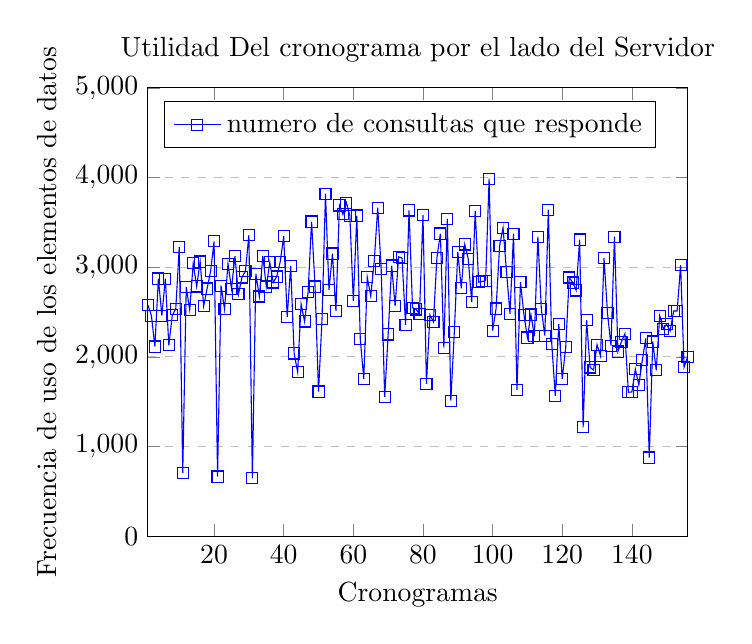
\begin{tikzpicture}
\begin{axis}[
    title={Utilidad Del cronograma por el lado del Servidor},
    xlabel={Cronogramas},
    ylabel={Frecuencia de uso de los elementos de datos},
    xmin=1, xmax=156,
    ymin=0, ymax=5000,
    xtick={},
    ytick={},
    legend pos=north west,
    ymajorgrids=true,
    grid style=dashed,
]

\addplot[
    color=blue,
    mark=square,
    ]
    coordinates {
%UTILIDAD TOTAL
%(cronograma, numero cues que usan al cronograma)
(1,2578)
(2,2459)
(3,2115)
(4,2873)
(5,2460)
(6,2871)
(7,2128)
(8,2463)
(9,2538)
(10,3226)
(11,702)
(12,2780)
(13,2523)
(14,3043)
(15,2785)
(16,3063)
(17,2566)
(18,2762)
(19,2954)
(20,3288)
(21,665)
(22,2793)
(23,2532)
(24,3040)
(25,2760)
(26,3124)
(27,2698)
(28,2886)
(29,2955)
(30,3357)
(31,645)
(32,2928)
(33,2673)
(34,3126)
(35,2784)
(36,3054)
(37,2830)
(38,2896)
(39,3062)
(40,3345)
(41,2443)
(42,3015)
(43,2038)
(44,1831)
(45,2588)
(46,2395)
(47,2719)
(48,3509)
(49,2784)
(50,1613)
(51,2421)
(52,3820)
(53,2747)
(54,3152)
(55,2512)
(56,3689)
(57,3589)
(58,3719)
(59,3574)
(60,2623)
(61,3576)
(62,2196)
(63,1751)
(64,2888)
(65,2678)
(66,3067)
(67,3664)
(68,2980)
(69,1551)
(70,2250)
(71,3018)
(72,2569)
(73,3116)
(74,3101)
(75,2353)
(76,3633)
(77,2546)
(78,2529)
(79,2480)
(80,3580)
(81,1700)
(82,2468)
(83,2391)
(84,3105)
(85,3375)
(86,2102)
(87,3538)
(88,1511)
(89,2275)
(90,3171)
(91,2764)
(92,3254)
(93,3094)
(94,2610)
(95,3626)
(96,2832)
(97,2842)
(98,2848)
(99,3987)
(100,2292)
(101,2539)
(102,3235)
(103,3441)
(104,2946)
(105,2480)
(106,3374)
(107,1630)
(108,2834)
(109,2470)
(110,2215)
(111,2472)
(112,2232)
(113,3341)
(114,2530)
(115,2237)
(116,3641)
(117,2141)
(118,1564)
(119,2364)
(120,1755)
(121,2109)
(122,2885)
(123,2829)
(124,2741)
(125,3308)
(126,1215)
(127,2409)
(128,1882)
(129,1853)
(130,2136)
(131,2009)
(132,3102)
(133,2487)
(134,2125)
(135,3341)
(136,2059)
(137,2169)
(138,2257)
(139,1605)
(140,1608)
(141,1861)
(142,1687)
(143,1963)
(144,2206)
(145,877)
(146,2171)
(147,1849)
(148,2460)
(149,2313)
(150,2362)
(151,2290)
(152,2512)
(153,2511)
(154,3024)
(155,1883)
(156,2000)
(157,2131)
    };
    \legend{numero de consultas que responde}

\end{axis}
\end{tikzpicture}

